\section{Diseño y Ensamblado}
\frame{
	\frametitle{Outline}
	\tableofcontents[currentsection]
	}

\subsection*{PyID}
% Una subsection* crea un nuevo "grupo de puntos"

\frame{
	\frametitle{PyID}

	\begin{center}
		\textbf{Definición}

		\vspace{0.25cm}

		\missingfigure[figwidth=6cm]{Figura completa}
	\end{center}

	\begin{columns}
		\begin{column}{0.5\textwidth}
			\begin{itemize}
				\item {\color{newcolor} Texto en columna 1}:
				\begin{itemize}
					\item item 1
					\item item 2
				\end{itemize}
				\item {\color{newcolor} Más texto}
			\end{itemize}
		\end{column}

		\begin{column}{0.5\textwidth}
			\begin{itemize}
				\item {\color{softBlue!70!Black} Texto:}
					en otra columna
				\item {\color{softOrange!70!Black} Más texto:}
					en otra columna
			\end{itemize}

		\end{column}
	\end{columns}
}

\subsection*{Circuito hidráulico}
\frame{
	\frametitle{Cañerías y Tanques}
	\begin{columns}
		\begin{column}{0.4\textwidth}
			\begin{enumerate}
				\item Una
				\begin{itemize}
					\item \textbf{Larga}
					\item larga
				\end{itemize}
				\item Lista
			\end{enumerate}

			\begin{align*}
				\mathrm{una} \,e( \textbf{cuacion})
			\end{align*}
		\end{column}

		\begin{column}{0.6\textwidth}
			\begin{center}
				\missingfigure[figwidth=4.5cm]{}
			\end{center}

			\begin{center}
				\footnotesize
				\textbf{\textit{Cita bibliográfica}}

				[Escrita por alguien \textit{et al.} 2008]
			\end{center}
		\end{column}

	\end{columns}
}

\frame{
	\frametitle{Bombas}
	\textbf{Idea:} ...
	\vspace{0.25cm}
	\begin{center}

		Lorem ipsum dolor sit amet, consectetur adipiscing elit.
		Donec viverra cursus pellentesque. In et mattis augue.
		Dorbi ut velit a ante ultrices ornare in id nisl.

		\vspace{0.5cm}

		Pellentesque sollicitudin bibendum leo lobortis sagittis.
		Fusce eu purus vel mauris vestibulum mattis.
	\end{center}
}
\subsection*{Válvula globo, con servoactuador de diafragma - resorte}
\frame{
	\frametitle{Válvula globo con servoactuador de diafragma - resorte}

	\textbf{Generalidades}
	\vspace{0.25cm}
	\begin{center}
		
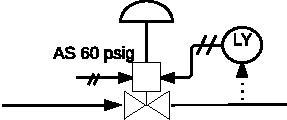
\includegraphics[scale=1]{Sections/2-DisenoEnsamblado/Images/ValvPyID.pdf}

	\vspace{0.25cm}

	Es un elemento central en nuestra planta, es la encargada de 
efectuar las acciones de control
	\end{center}

	\begin{columns}[t]
		\begin{column}{0.5\textwidth}
			\begin{itemize}
				\item {\color{newcolor} Características}:
				\begin{itemize}
					\item Válvula Isoporcentual
					\item Aire para abrir (NC)
					\item Con electroposicionador
				\end{itemize}
			\end{itemize}
		\end{column}

		\begin{column}{0.5\textwidth}
			\begin{itemize}
				\item {\color{newcolor} Entradas}:
				\begin{itemize}
				 \item Aire: $4\,bar$
				 \item Señal: $4$ - $20\,mA$
				\end{itemize}

			\end{itemize}

		\end{column}
	\end{columns}
}

\frame{
	\frametitle{Válvula globo, con servoactuador de diafragma - resorte}

	\textbf{Principio de Funcionamiento}
	\begin{columns}[t]
		\begin{column}{0.5\textwidth}
		\begin{center}
		 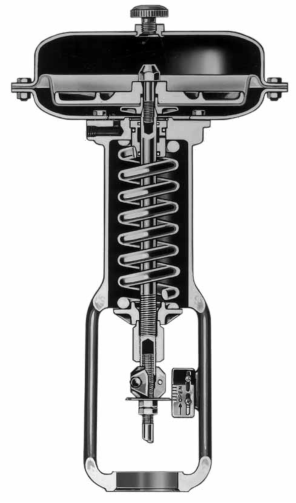
\includegraphics[width=.6\textwidth]
{Sections/2-DisenoEnsamblado/Images/ActuadorValvNeum.pdf}
 \footnotesize
 
       Actuador Neumático Inverso
		\end{center}


		\end{column}

		\begin{column}{0.5\textwidth}
		
		\begin{center}
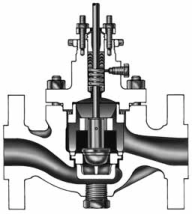
\includegraphics[width=.6\textwidth]
{Sections/2-DisenoEnsamblado/Images/ValvGlob.pdf}

 \footnotesize
       Cuerpo de la válvula
       
       Conjunto asiento-obturador
\end{center}
		\begin{itemize}
		 \item Convertidor I/P, presión de aire comprimido ($3$ - 
$15\,psi$)
		\item Equilibrio presión aire - resorte
		\end{itemize}
		\end{column}

	\end{columns}
}
\frame{
	\frametitle{Válvula globo, con servoactuador de diafragma - resorte}
	\begin{center}
	 	\textbf{Curvas características}
	\end{center}
	\vspace{0.25cm}
	\begin{columns}[t]
		\begin{column}{0.5\textwidth}
		\textbf{Caract. caudal inherente}
		
		Relaciona carrera-caudal, a $\Delta p$ cte.
		\begin{center}
		 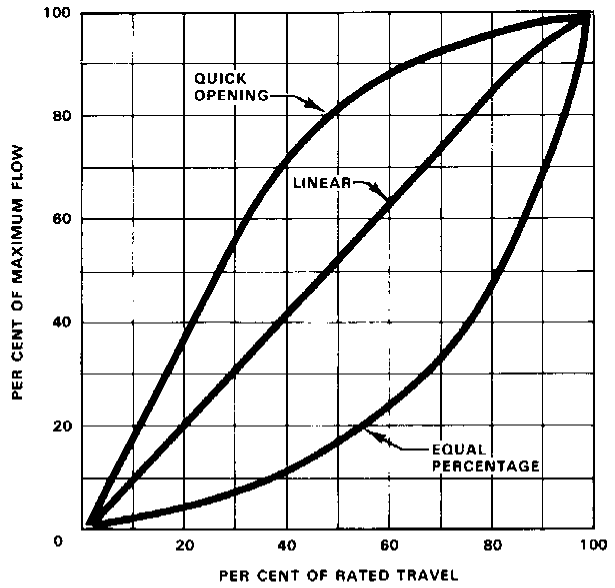
\includegraphics[width=.9\textwidth]
{Sections/2-DisenoEnsamblado/Images/Inherente.png}
 \footnotesize
		\end{center}
% 		\begin{itemize}
% 		 \item Lineal
% 		 \begin{align*}
% 		  q = k\,l
% 		 \end{align*}
% 		 \item Isoporcentual
% 		 \begin{align*}
% 		  \dfrac{q_{max}}{q_{min}} = e^a
% 		 \end{align*}
% 		 \item Quick Opening
% 		\end{itemize}


		\end{column}

		\begin{column}{0.5\textwidth}
		\textbf{Caract. caudal efectiva}
		
		Idem, a $\Delta p$ variable
		
		\begin{figure}[ht]
  \centering
  \resizebox {\columnwidth} {!} {
  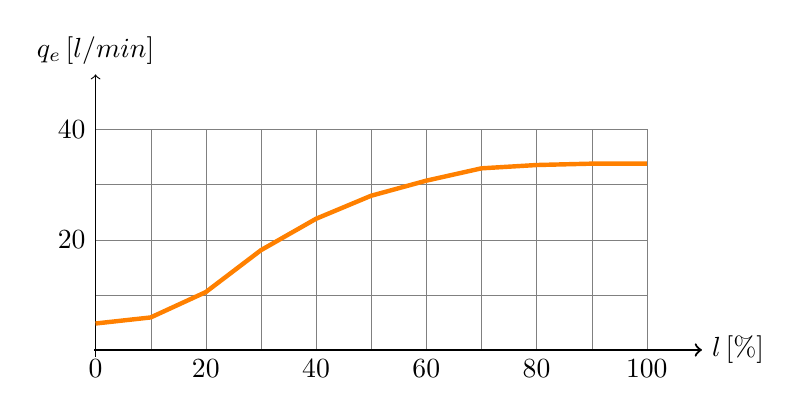
\begin{tikzpicture}[scale=.07,domain=0:110]
    
    \draw[ultra thin,color=gray,step=10cm] (100,40) grid (0.1,0.1);
    \draw[thick,->] (-0.2,0) -- (110,0) node[right,draw=none] {$l\,[\%]$};
    \draw[->] (0,-1.2) -- (0,50) node[above,draw=none] {$q_e\,[l/min]$};
    
    \foreach \x in {0,20,40,60,80,100}
    \draw (\x cm,1pt) -- (\x cm,-1pt) node[anchor=north,draw=none] {$\x$};
    \foreach \y in {20,40}
    \draw (1pt,\y cm) -- (-1pt,\y cm) node[anchor=east,draw=none] {$\y$};
    
    \draw[color = orange,ultra thick] (0,4.8) -- (10,5.9) -- (20,10.5)
    -- (30,18.1) -- (40,23.8) -- (50,27.98) -- (60,30.71)
    -- (70,32.95) -- (80,33.55) -- (90,33.8) -- (100,33.82);
   
	\end{tikzpicture}
	}
	\end{figure}
% 	\begin{itemize}
% 	 \item Linealidad en la zona de trabajo
% 	 \item Efecto del flujo estrangulado
% 	\end{itemize}
	\vspace{-.5cm}
	\begin{align*}
	 q_e &= \dfrac{1}{\sqrt{1-r+\dfrac{r}{{q_i}^2}}}
	\end{align*}


	\end{column}

	\end{columns}
}

\frame{
	\frametitle{Válvula globo, con servoactuador de diafragma - resorte}
	\textbf{Electroposicionador}
	
	\vspace{.25cm}
	
	{\color{newcolor} Problema:} en convertidor I/P no hay \textbf{real 
comparación} entre la consigna y la posición del vástago

	\begin{columns}
	 \begin{column}{.35\textwidth}
	  {\color{newcolor2} Soluciona:}
	  \begin{itemize}
	   \item Fricciones en vástago
	   \item Fuerzas dinámicas
	   \item Perturbaciones
	  \end{itemize}

	 \end{column}
	 \begin{column}{.65\textwidth}
	  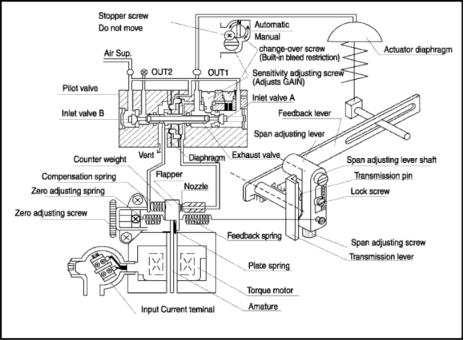
\includegraphics[width=\textwidth]
{Sections/2-DisenoEnsamblado/Images/PG-EPL.pdf}
	 \end{column}
	\end{columns}
}

\subsection*{Instrumentación}
\frame{
	\frametitle{Placa Orificio}
	\begin{columns}
		\begin{column}{0.4\textwidth}
			\begin{enumerate}
				\item Una
				\begin{itemize}
					\item \textbf{Larga}
					\item larga
				\end{itemize}
				\item Lista
			\end{enumerate}

			\begin{align*}
				\mathrm{una} \,e( \textbf{cuacion})
			\end{align*}
		\end{column}

		\begin{column}{0.6\textwidth}
			\begin{center}
				\missingfigure[figwidth=4.5cm]{}
			\end{center}

			\begin{center}
				\footnotesize
				\textbf{\textit{Cita bibliográfica}}

				[Escrita por alguien \textit{et al.} 2008]
			\end{center}
		\end{column}

	\end{columns}
}

\frame{
	\frametitle{DP Cells}
	\textbf{Idea:} ...
	\vspace{0.25cm}
	\begin{center}

		Lorem ipsum dolor sit amet, consectetur adipiscing elit.
		Donec viverra cursus pellentesque. In et mattis augue.
		Dorbi ut velit a ante ultrices ornare in id nisl.

		\vspace{0.5cm}

		Pellentesque sollicitudin bibendum leo lobortis sagittis.
		Fusce eu purus vel mauris vestibulum mattis.
	\end{center}
}
\frame{
	\frametitle{Manómetros}
	\textbf{Idea:} ...
	\vspace{0.25cm}
	\begin{center}

		Lorem ipsum dolor sit amet, consectetur adipiscing elit.
		Donec viverra cursus pellentesque. In et mattis augue.
		Dorbi ut velit a ante ultrices ornare in id nisl.

		\vspace{0.5cm}

		Pellentesque sollicitudin bibendum leo lobortis sagittis.
		Fusce eu purus vel mauris vestibulum mattis.
	\end{center}
}
